\documentclass[10pt,twocolumn,journal]{IEEEtran}
% XeLaTeX: all fonts are resolved from the local installation.
\usepackage{fontspec}
\defaultfontfeatures{Ligatures=TeX}
\setmainfont[
  BoldFont=TeXGyreTermes-Bold,
  ItalicFont=TeXGyreTermes-Italic,
  BoldItalicFont=TeXGyreTermes-BoldItalic,
  SmallCapsFont=TeXGyreTermes-Regular,
  SmallCapsFeatures={Letters=SmallCaps}
]{TeXGyreTermes-Regular}
\IfFontExistsTF{Arial}{\setsansfont{Arial}}{\setsansfont{Liberation Sans}}
\setmonofont{TeXGyreCursor-Regular}

\usepackage[margin=1in,bottom=1.12in]{geometry}
\usepackage{xeCJK}
% Build script resolves installed standalone Chinese font files.
% The generated file contains local font paths only; no font binaries are distributed.
\InputIfFileExists{../font_local_zh.tex}{}{%
  \setCJKmainfont[BoldFont=FandolSong-Bold.otf,ItalicFont=FandolKai-Regular.otf,SmallCapsFont=FandolSong-Regular.otf]{FandolSong-Regular.otf}
  \setCJKsansfont[BoldFont=FandolHei-Bold.otf]{FandolHei-Regular.otf}
  \setCJKmonofont{FandolFang-Regular.otf}
}

\usepackage{amsmath,amssymb}
\usepackage{booktabs,array,multirow}
\usepackage{graphicx}
\usepackage{xurl}
\usepackage{xr-hyper}
\usepackage[hidelinks,unicode]{hyperref}
\urlstyle{same}
\usepackage{fancyhdr}
\usepackage{flushend}
\externaldocument{supplement}[supplement.pdf]
\graphicspath{{figures/}}
\setlength{\emergencystretch}{4em}
\renewcommand{\figurename}{图}
\renewcommand{\tablename}{表}
\renewcommand{\refname}{参考文献}
\renewcommand{\abstractname}{摘要}
\renewcommand{\IEEEkeywordsname}{关键词}
\DeclareMathOperator{\NLL}{NLL}
\DeclareMathOperator{\CRPS}{CRPS}
\DeclareMathOperator{\Std}{std}
\pagestyle{fancy}
\fancyhf{}
\fancyhead[L]{\scriptsize BELOW ZERO}
\fancyhead[R]{\scriptsize\thepage}
\renewcommand{\headrulewidth}{0pt}
\hypersetup{pdftitle={Below Zero：面向下限删失 RAW 图像的空间自适应条件读出抽样},pdfauthor={},pdfsubject={中文学术译稿，与最终英文编辑稿对应}}
\newcommand{\BZAuthorBlockEN}{Yaogeng Jiang\\Independent Researcher\\\href{mailto:y.g.jiang@sjtu.edu.cn}{y.g.jiang@sjtu.edu.cn}}
\newcommand{\BZAuthorBlockZH}{姜尧耕\\独立研究者\\\href{mailto:y.g.jiang@sjtu.edu.cn}{y.g.jiang@sjtu.edu.cn}}
\newcommand{\BZPDFAuthors}{Yaogeng Jiang}

\hypersetup{pdfauthor={\BZPDFAuthors}}
\begin{document}
\title{{\normalsize \href{https://github.com/y-g-jiang/Video-RAW-Black-Level-Correction-Net/tree/main/below_zero}{代码与数据}}\\[6pt]Below Zero：面向下限删失 RAW 图像的\\空间自适应条件读出抽样}
\author{\BZAuthorBlockZH}
\maketitle
\thispagestyle{fancy}

\begin{abstract}
在黑电平扣除后将 RAW 传感器测量值在零处截断，会丢弃负值读出码并使暗部统计产生正偏。本文提出一种单帧条件补全方法 N0/PG，在原样保留所有正测量值的同时，仅于下限删失位置抽取有符号整数读出。该方法利用多尺度卷积估计器预测局部信号水平，再由经校准的量化 Poisson--Gaussian（PG）解码器将各位置预测映射为零码及负整数码的条件概率分布，因此将补全后的 Bayer 图像在零处重新截断即可无损还原输入。在校准的高增益传感器模型下，N0/PG 在 138 幅留出测试源图上相对于局部最大似然估计将平均超额 Kullback--Leibler（KL）散度从 0.001723 降至 0.000313 nats（全部 138 幅源图的 KL 均获改善），并将留出整数码的负对数似然（NLL）每删失像素降低 0.001407 nats。分区域分析表明，经典局部估计器在均匀近黑区域已较准确，而多尺度上下文的优势主要体现在较高信号水平与非均匀结构邻域。在保持预测分布集合不变的条件下随机打乱其空间位置会使误差显著回升，证实了空间位置分配的关键作用。在两组保留黑电平以下有符号参考读出的实拍曝光及受控色彩渲染实验中，条件读出抽样均有效恢复了被截断压制的去马赛克暗部起伏并减轻暗部偏色。上述结果建立了一种测量保持的下限删失 RAW 补全框架，并量化了学习式空间估计对条件读出分布精度的贡献。
\end{abstract}

\begin{IEEEkeywords}
计算成像，删失测量，Bayer RAW 图像，Poisson--Gaussian 噪声，概率重建，去马赛克。
\end{IEEEkeywords}

\section{引言与相关工作}
相机成像管线在扣除标称黑电平后，使 RAW 传感器读出围绕有符号原点分布。即便入射光信号恒为非负，电子读出噪声仍会在暗区产生负整数码。将这些负码在零点截断会改变观测噪声的均值与方差 \cite{foi2008,foi2009}，进而影响后续空间平均与插值。此类下限截断广泛见于有文档记录的相机处理管线 \cite{mathworksISP}、相机 RAW 文件调查 \cite{librawD5300,claffReadNoise}，以及 AIM 2025 低光 RAW 视频挑战赛中 VMCL-ISP 团队分析的负噪声截断 \cite{aim2025Video}，同时标准 RAW 评价接口也普遍施加非负输出约束 \cite{sonyAIM2025}。

本文的目标是从单幅下限删失 Bayer 图像出发，补全统计合理的有符号整数读出样本。零点截断将原生零码与所有负整数码合并为同一观测值 $Y_i=0$。不同于输出去噪信号估计的复原任务，测量保持补全仅在删失像素处抽取非正整数码，同时严格保持所有正测量值不变，从而为下游处理保留完整的传感器域测量表示。

核心挑战在于，相同的零观测在不同空间位置未必对应相同的条件读出分布。明亮边缘旁的零码与均匀暗区内的零码，对被截断读出蕴含着截然不同的统计证据。邻近未删失的正测量值携带着这一结构差异，但局部常值信号模型在跨越边缘时容易将其平滑抹去。一旦利用周围上下文估计出空间变化的信号场，同一个校准物理解码器便能为不同结构邻域赋予相应的条件读出概率分布。

为此，N0/PG 将空间信号估计与物理条件解码解耦（图~\ref{fig:pipeline}）。NAF 风格卷积网络 \cite{nafnet} 根据打包 Bayer 观测与校准常量预测非负信号场，经校准的量化 Poisson--Gaussian（PG）解码器再计算给定 $Y_i=0$ 时零码及各负整数码的条件分布。采样器仅填充删失像素，而恒等分支将每个正测量值原样复制通过。

\begin{figure*}[t]
\centering
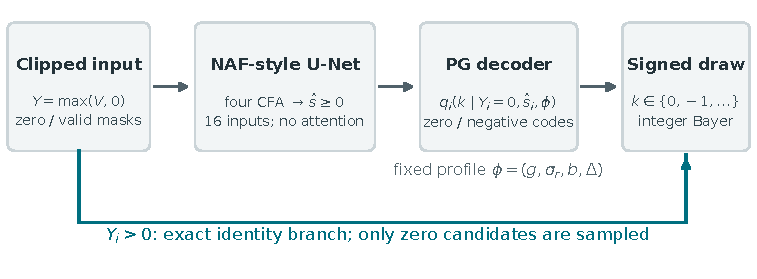
\includegraphics[width=\textwidth]{f01_pipeline.pdf}
\caption{空间自适应有符号 RAW 补全流程。网络为量化 PG 解码器预测局部信号参数，删失位置从零观测对应的非正整数条件分布中抽样，已观测正码则经恒等分支原样通过。}
\label{fig:pipeline}
\end{figure*}

本文考察学习式空间上下文能否比局部噪声模型拟合与变换域滤波更准确地估计条件读出分布。我们在 138 幅留出源图上评估分布精度，剖析收益随信号强度与邻域结构的变化规律，并检验补全有符号样本对去马赛克与固定色彩渲染的影响。

\subsection{相关工作}
\subsubsection{删失测量与 RAW 噪声模型}
条件插补是处理删失观测的经典方法。在 Tobit 回归中，O'Neill \cite{oneill2024} 采用潜在数据增强，在保留未删失响应的同时从条件分布中抽取删失响应。在计算成像中，Kodgirwar 等人 \cite{kodgirwar2024} 针对多曝光叠层成像融合推断饱和 Poisson 光子计数。本文将条件读出补全引入受量化 PG 噪声干扰的单幅 Bayer 图像，同时保留实测正码与原生零码的离散概率质量。

Foi 等人 \cite{foi2008} 建立了包含截断效应的实用 RAW 图像 PG 噪声模型，随后 Foi \cite{foi2009} 推导了方差稳定变换与逆偏差校正以实现截断异方差观测去噪。本文的条件解码器正是建立在该统计模型之上，但传统去噪旨在估计潜在无噪信号，而本文旨在恢复删失像素处的整数读出。为实现公平对比，Foi-qPG 基线先执行上述截断变换与协同滤波，再接入与其余估计器相同的量化条件解码器（第~\ref{sec:baselines} 节）。

真实传感器还存在独立高斯读出噪声之外的非理想效应。Wei 等人 \cite{wei2020} 建模了极弱光下的重尾与条带噪声分量，Zhang 等人 \cite{zhang2021} 探讨了相关噪声与量化效应，Mohammadi 等人 \cite{mohammadi2026} 研究了黑电平偏差引起的暗部偏色。即便正码与零观测事件不变，这些效应仍可能改变缺失负码的尾部形态。

\subsubsection{学习式估计与条件抽样}
NAFNet \cite{nafnet} 提供了高效的图像复原卷积模块。本文实现了一个不含全局池化通道注意力的四阶段 NAF 风格编码器与解码器网络，使估计器具有严格有界的空间感受野。网络仅输出以数字单位（DN）表示的非负信号参数，具体读出概率则由校准 PG 模型决定。

将学习先验与物理测量模型结合已广泛用于深度平衡重建 \cite{gilton2021}、神经网络凸正则化 \cite{goujon2023} 与深度生成先验贝叶斯反演 \cite{bohra2022}。这些方法致力于恢复潜在干净图像，而本文推断的是给定零观测时被截断的整数读出。受 Gnanasambandam 等人关于非盲 Poisson 反卷积分析 \cite{gnanasambandam2024} 的启发，本文独立考察空间信号估计器的作用，并采用严格恰当评分规则 \cite{gneiting2007} 定量评估预测的条件分布。

\subsubsection{去马赛克与下游处理}
联合去马赛克与去噪方法利用空间和跨通道相关性直接恢复干净彩色图像 \cite{gharbi2016}。本文任务位于成像管线更前端，即在色彩插值前恢复统计自洽的有符号传感器测量。为在不引入学习式后处理干扰的前提下检验其影响，我们采用自适应同质性导向（AHD）去马赛克算法 \cite{hirakawa2005} 的固定 LibRaw 实现 \cite{libraw}。

\section{条件读出补全}
\subsection{量化的下限删失读出}
令 $s_i\geq0$ 为像素 $i$ 处以 DN 表示的期望光学信号，$g$ 为以 DN/e$^{-}$ 为单位的转换增益，$b_i$ 为相对标称黑电平的已知偏移。在校准 PG 模型下，光电子计数 $N_i$ 与连续有符号读出 $Z_i$ 满足
\begin{align}
N_i&\sim\operatorname{Poisson}(s_i/g),\label{eq:pois}\\
Z_i&=gN_i+b_i+\epsilon_i,\qquad \epsilon_i\sim\mathcal N(0,\sigma_r^2).\label{eq:forward}
\end{align}
以 1 DN 步长作最近整数量化得到 $V_i=\lfloor Z_i+1/2\rfloor$。选取统一的有符号码原点即可将截断下限写为零（文件域中位于其他码值的下限可通过平移该原点等价表示）。下限删失随后产生
\begin{equation}
Y_i=\max(V_i,0),\qquad \mathcal Z=\{i:Y_i=0\}.\label{eq:censor}
\end{equation}
模拟器包含 $16383-512=15871$ DN 的上限饱和。所有纳入评估的样本均保持在 ADC 物理下界之上，在此工作范围内读出噪声由无界高斯分布刻画。

对于任意非正整数 $k\leq0$，量化码值 $k$ 的无条件概率质量为
\begin{align}
a_k(s,b)=\sum_{n=0}^{\infty}\operatorname{Pois}(n;s/g)
\bigg[&\Phi\!\left(\frac{k+1/2-gn-b}{\sigma_r}\right)\nonumber\\[-2pt]
-&\Phi\!\left(\frac{k-1/2-gn-b}{\sigma_r}\right)\bigg],\label{eq:bin}
\end{align}
其中 $\Phi$ 为标准正态累积分布函数。观测到零码（$Y_i=0$）的总概率为
\begin{equation}
c(s,b)=\sum_{n=0}^{\infty}\operatorname{Pois}(n;s/g)
\Phi\!\left(\frac{1/2-gn-b}{\sigma_r}\right).\label{eq:zeroevent}
\end{equation}
这里 $+1/2$ DN 积分上界同时涵盖了原生零码的量化区间与所有负整数码的量化区间。

给定信号估计 $\hat s_i$，物理解码器返回条件读出分布
\begin{equation}
q_i(k)=\frac{a_k(\hat s_i,b_i)}{c(\hat s_i,b_i)},\qquad k=0,-1,-2,\ldots.\label{eq:posterior}
\end{equation}
式~\eqref{eq:bin} 的单位区间积分保留了 $k=0$ 处的离散概率原子，而式~\eqref{eq:posterior} 的归一化则以完整零观测事件 $V_i\leq0$ 为条件。图~\ref{fig:counterexamples} 展示了该条件分布如何随局部图像结构变化。

\subsection{测量保持补全}
对每个零值候选位置 $i\in\mathcal Z$，从其预测条件分布 $q_i$ 中抽取 $K_i$，构造补全输出
\begin{equation}
\widetilde V_i=\begin{cases}
Y_i,&Y_i>0,\\
K_i,\quad K_i\sim q_i,&Y_i=0.
\end{cases}\label{eq:output}
\end{equation}
恒等分支与 $q_i$ 的非正支撑集保证 $\max(\widetilde V_i,0)=Y_i$ 精确成立。条件样本旨在表达被截断抹去的含噪读出起伏，而非无噪信号的点估计，因此随机抽样与条件均值插补对应不同损失目标。本文采用恰当概率评分规则评价预测分布 $q_i$，随机抽样与条件均值的平方误差风险恒等式见补充材料第 I 节。

当模拟信号 $s_i$ 已知时，前向模拟器提供已知信号参考分布
\begin{equation}
p^{\star}_i(k)=a_k(s_i,b_i)/c(s_i,b_i),\label{eq:oracle}
\end{equation}
而在推理阶段，解码器将预测信号场 $\hat s_i$ 代入式~\eqref{eq:posterior} 得到条件分布 $q_i$，并在给定 $\hat s_i$ 条件下跨像素独立抽样。

\section{学习空间自适应读出分布}
\subsection{信号估计器}
我们将 Bayer 四个相位打包为 $[R,G_1,G_2,B]$，向网络输入经变换的测量图、零候选二值指示图、已知偏移、空间有效性掩码与校准常量。有效性掩码区分边界填充与实测零码，已知偏移则同时输入信号估计器与 PG 解码器。

四阶段 NAF 风格编码器与解码器通过加性跳跃连接与像素重排上采样融合多尺度特征。逐位置跨通道归一化、深度卷积与乘性门控构成有界空间感受野，不含全局池化或自注意力。四通道 softplus 输出头预测以 DN 表示的 $\hat s_i\geq0$，再按光电子均值 $\hat s_i/g$ 送入解码器。模型共含 10,913,380 个参数，输入通道定义与各阶段维度见补充材料第 II 节。

\subsection{以条件分布为目标进行训练}
合成训练直接利用真实信号 $s_i$ 构造参考条件分布 $p_i^\star$，并在有效零值候选集合 $\mathcal Z$ 上最小化条件交叉熵：
\begin{equation}
\mathcal L(\theta)=-\frac{1}{|\mathcal Z|}
\sum_{i\in\mathcal Z}\sum_{k\leq0}p^{\star}_i(k)\log q_{\theta,i}(k).
\label{eq:loss}
\end{equation}
数值实现在包含显式下尾类别的有限离散支撑集上计算式~\eqref{eq:loss}。由于目标熵 $H(p_i^\star)$ 与网络参数 $\theta$ 无关，最小化该交叉熵等价于最小化相对于已知信号参考分布的 KL 散度。梯度经可微物理解码器反向传回网络，使信号预测直接针对删失读出分布精度进行优化。由于校准常量与逐样本偏移均作为已知输入提供给解码器，训练仅更新空间估计器权重。

\subsection{离散分布的数值计算与坐标索引抽样}
离散表示显式保留 $0,-1,\ldots,-304$，并将 $V\leq-305$ 合并为一个下尾类别。在计算整数对数似然、CRPS 及执行抽样时，落入下尾类别的事件会进一步解析到单个负整数码。条件尾部解析公式、查找表插值误差界与坐标索引抽样详见补充材料第 III 节。

\begin{figure*}[t]
\centering
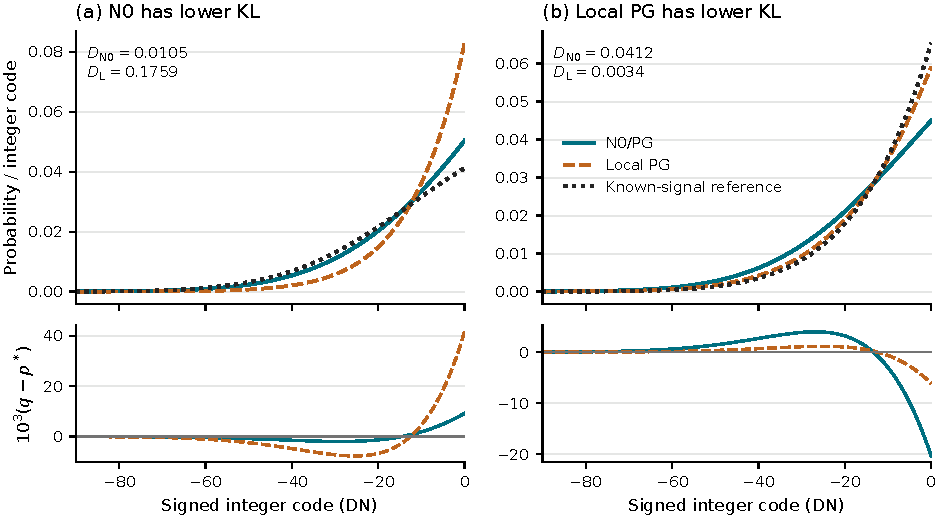
\includegraphics[width=\textwidth]{f02_pmf_counterexamples.pdf}
\caption{开发集两个高梯度位置的条件 PMF（于评估后选取，用于展示两类方法在不同局部结构下各有优势的情形）。上排展示 N0/PG、Local PG 与已知信号分布，下排展示有符号概率误差。N0 在（a）中更准确，Local PG 在（b）中更准确。}
\label{fig:counterexamples}
\end{figure*}

\section{实验}
\subsection{数据、校准与训练}
实验采用 Panasonic S5 II 在 ISO12800 下的实测校准参数（表~\ref{tab:protocol}）。增益 $g$ 来自光子转移（JOT）测量 \cite{jot}，读出噪声由十幅暗帧的 R 与 $G_1$ 相位联合标定。合成信号生成、已知信号参考分布与条件解码器共用同一 PG 模型，使留出测试能够纯粹衡量匹配噪声物理下的空间条件分布估计，而保留真实负码的暗室曝光则用于检验该模型在真实读出上的表现。

\begin{table}[t]
\centering\small
\caption{传感器校准参数与实验设置。}
\label{tab:protocol}
\begin{tabular}{@{}p{0.40\columnwidth}p{0.52\columnwidth}@{}}
\toprule
项目 & 设置\\
\midrule
传感器设置 & S5 II，ISO12800，机械快门，14 bit\\
增益 $g$ & 21.6010924121 DN/e$^{-}$\\
整数读出噪声 RMS & 24.9612744275 DN\\
模拟域 $\sigma_r$ & 24.9596051193 DN\\
标称黑电平 / 步长 & 512 DN / 1 DN\\
合成偏移 $b_c$ & 已知，均匀分布于 $[-0.25,0.25]$ DN\\
源图像划分 & 825 训练 / 137 开发 / 138 测试\\
训练 & Seed 7103，80,000 次更新\\
测试上下文 / 目标核心 & 128 和 256 / 中心 64 个打包像素\\
\bottomrule
\end{tabular}
\end{table}

合成信号场由 DIV2K 和 BSDS500 的 1,100 幅彩色模板 \cite{div2k,bsds500} 生成，按源图划分为 825 幅训练、137 幅开发与 138 幅留出测试图像。训练样本中自然场景占 90\%，程序化控制占 10\%，其曝光缩放、颜色扰动、量化与截断按补充材料第 II 节执行。单次训练得到的 N0 模型依据开发集选定冻结。

每幅留出源图生成两个曝光与噪声实现不同的测试场景，并分别在共享中心 64 像素目标区的 128 与 256 打包像素上下文中评估。138 幅源图共产生 552 个案例和 3,254,612 个评分条目（其中 256 像素上下文包含 1,627,306 个唯一候选位置）。

\subsection{对比方法}\label{sec:baselines}
Global PMF 对每个 CFA 相位采用训练集统计的平均条件分布，Global PG 则将训练集拟合的逐相位常数信号代入校准解码器，两者在测试时均给出空间恒定预测。

Local PG 在同相位 $5\times5$ 邻域内综合正码与零码删失事件的似然进行最大似然信号拟合，而 Local Bayes 在此似然基础上结合训练集拟合的零点加 Gamma 信号先验，对条件分布进行后验积分。两者均使用开发集选定的 $5\times5$ 窗口，且中心零观测仅计入一次。

Foi-qPG 基于 Foi 的截断噪声正变换 \cite{foi2009} 与 BM3D 滤波 \cite{bm3d} 构建，经量化 PG 逆变换后接入共享的条件整数解码器。

N0 联合利用四个 CFA 相位提取多尺度特征，而主要局部基线仅使用同相位观测。开发集 Joint-CFA Bayes 对照同样在 $5\times5$ 窗口内联合利用四个相位，用于检验局部跨相位观测能否弥合误差差距（补充材料第 VII-A 节）。

\subsection{评价准则}
对每个保留作参考的有符号整数码 $v_i$，我们采用负对数似然（NLL）与离散连续秩概率评分（CRPS）评价预测分布 $q_i$：
\begin{align}
\NLL(q_i,v_i)&=-\log q_i(v_i),\label{eq:nll}\\
\CRPS(q_i,v_i)&=\sum_{k\in\mathbb Z}
\left(F_{q_i}(k)-\mathbf{1}\{v_i\leq k\}\right)^2\Delta.\label{eq:crps}
\end{align}
这里 NLL 单位为每候选像素 nats，CRPS 单位为 DN（步长 $\Delta=1$ DN），两者均按实际隐藏整数码求值并解析下尾类别内的具体整数码。

模拟信号已知时，还可通过超额 KL 散度与累积分布平方差异直接比较预测分布与已知信号参考分布：
\begin{align}
D_i&=\sum_{k\leq0}p^{\star}_i(k)\log\frac{p^{\star}_i(k)}{q_i(k)},\label{eq:kl}\\
J_i&=\sum_{k\in\mathbb Z}\left(F_{q_i}(k)-F_{p^{\star}_i}(k)\right)^2\Delta.\label{eq:cdf}
\end{align}
超额 KL 与 $J_{\mathrm{CDF}}$ 在包含聚合下尾类别的 306 类共同表示上计算，NLL 与 CRPS 则解析整数尾部（数值误差界见补充材料第 III 节）。

各评分先在源图内部汇总，再对源图等权平均。成对源图 bootstrap 将同一源图的关联案例捆绑重采样。针对 Local Bayes 和 Foi-qPG 的两项预注册主 KL 对比采用 97.5\% 置信区间，其余对比采用 95\% 区间（补充材料第~\ref{sec:scoreaggregation}、\ref{sec:regionaldefinitions} 节）。

\subsection{留出数据上的条件分布精度}
如表~\ref{tab:holdout} 所示，N0/PG 在所有可部署方法中取得最低的超额 KL、$J_{\mathrm{CDF}}$、NLL 和 CRPS。已知信号参考给出模拟器内的理论下界，而确定性零填充对负码赋予零概率，其 KL 与 NLL 为无穷大。

\begin{table*}[t]
\centering\small
\caption{138 幅留出源图上的条件分布评分，每幅源图含四个相关案例与上下文组合并按源图等权汇总。超额 KL 与 $J_{\mathrm{CDF}}$ 使用 306 类别，NLL 与 CRPS 分辨整数尾部。粗体表示最佳可部署方法。零填充对负标签赋予零概率，故 KL/NLL 为无穷大，而已知信号参考使用实际不可得的真实信号。}
\label{tab:holdout}
\begin{tabular}{@{}llrrrr@{}}
\toprule
方法 & 可用空间信息 & $10^3D_{\mathrm{KL}}\downarrow$ & NLL$\downarrow$ & CRPS$\downarrow$ & $10^3J_{\mathrm{CDF}}\downarrow$\\
\midrule
零填充 & 无 & $\infty$ & $\infty$ & 18.691235 & 10611.0233\\
Global PMF & 逐 CFA 训练分布律 & 3.4350 & 3.914828 & 8.112251 & 29.6469\\
Global PG & 逐 CFA 训练信号 & 3.3399 & 3.914723 & 8.111302 & 28.7879\\
Local PG & 同 CFA $5\times5$ & 1.7228 & 3.912975 & 8.095007 & 13.7075\\
Local Bayes & 同 CFA $5\times5$ & 1.8429 & 3.913102 & 8.096170 & 14.8024\\
Foi-qPG & 同 CFA 图像平面 & 2.1475 & 3.913454 & 8.100521 & 18.5915\\
\textbf{N0/PG（本文）} & 四 CFA 多尺度 & \textbf{0.3125} & \textbf{3.911568} & \textbf{8.084118} & \textbf{2.6423}\\
已知信号参考 & 不可得的真实信号 & 0.0000 & 3.911245 & 8.081423 & 0.0000\\
\bottomrule
\end{tabular}
\end{table*}

N0 减 Local Bayes 与 Foi-qPG 的主比较超额 KL 差值分别为 $-1.5304\times10^{-3}$ 和 $-1.8350\times10^{-3}$ nats，97.5\% 置信区间分别为 $[-2.1085,-1.0776]\times10^{-3}$ 与 $[-2.1474,-1.5372]\times10^{-3}$。相对于表现最强的局部基线 Local PG，N0 将平均超额 KL 从 $1.722793\times10^{-3}$ 降至 $3.125067\times10^{-4}$ nats，相对降幅达 81.86\%。

在留出整数码上，N0 相对于 Local PG 将平均 NLL 每候选像素降低 0.001407 nats（95\% 区间 $[-0.001950,-0.000969]$），CRPS 降低 0.010890 DN（95\% 区间 $[-0.014860,-0.007683]$）。超额 KL 的相对降幅远大于总 NLL，是因为期望对数损失包含无法由任何信号估计器消除的读出条件熵 $H(p_i^\star)$。图~\ref{fig:holdout} 展示了绝对评分与成对差异。

在全部 138 幅测试源图上，N0 均取得比 Local PG 更低的超额 KL（逐源图降幅中位数为 0.0004693 nats），并在 130 幅源图上取得更低 NLL、在 131 幅源图上取得更低 CRPS。

\begin{figure*}[t]
\centering
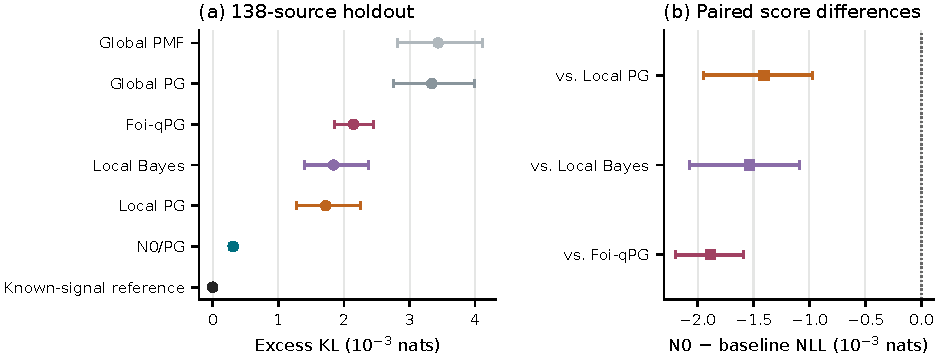
\includegraphics[width=\textwidth]{f03_holdout.pdf}
\caption{留出测试集的条件分布精度。（a）平均超额 KL 及 95\% 源图 bootstrap 区间。（b）相对于 N0 的成对 NLL 差值及 95\% 区间，其中负值有利于 N0。两项主比较的 97.5\% 区间见正文。}
\label{fig:holdout}
\end{figure*}

\subsection{信号强度与邻域结构的影响}\label{sec:regions}
明亮边缘附近的零码与均匀暗区内的零码在潜在信号和可见邻域线索上均有明显差异，因此空间估计的收益随局部结构而变。图~\ref{fig:spatial} 给出了超额 KL 随信号强度、局部变化度、边缘距离及观测零码比例的分区域对比（分箱定义见补充材料第~\ref{sec:regionaldefinitions} 节）。

\subsubsection{信号水平}
近黑区域的条件分布主要由标称读出噪声的负尾决定，不同信号估计给出的分布差异很小。相应地，N0 减 Local Bayes 的平均超额 KL 在 $s<0.25$ DN 时仅为 $-0.000087$ nats，而在 $8\leq s<16$ DN 时扩大至 $-0.002887$ nats。Foi-qPG 在 2 DN 以下的平均误差略低，而 N0 在 4 DN 以上显著优于所有基线（图~\ref{fig:spatial}(a)）。

\subsubsection{邻域变化}
误差差距随邻域结构变化而显著扩大，N0 减 Local Bayes 的超额 KL 差值从平坦区（$t<0.025$，含 115 幅源图的 379,366 个候选位置）的 $-0.000358$ nats 扩大至高变化区（$t\geq0.8$，含 106 幅源图的 98,229 个候选位置）的 $-0.004467$ nats。类似地，显著梯度位置处的差值为 $-0.002200$ nats，而距边缘至少 16 个打包像素处则为 $-0.000330$ nats。

按观测零码比例 $z$ 划分从测量端印证了同一规律，$z<0.1$ 时 N0 减 Local Bayes 的 KL 差值为 $-0.008058$ nats（17,450 个候选位置），而 $0.5\leq z<0.75$ 时收窄为 $-0.000226$ nats（498,135 个位置）。当删失像素周围大多为正测量值时，多尺度估计优势最大。由于信号强度与局部变化相关，第~\ref{sec:gradientcontrol} 节进一步在源图、CFA 相位和信号分箱内部进行匹配梯度对比。

\begin{figure*}[t]
\centering
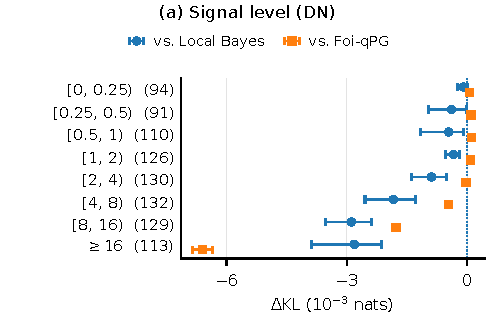
\includegraphics[width=0.493\textwidth]{f10a_holdout_signal.pdf}\hfill
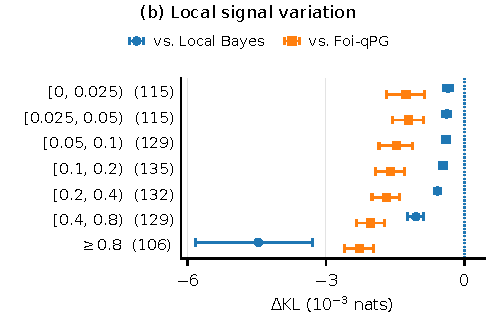
\includegraphics[width=0.493\textwidth]{f10b_holdout_variation.pdf}\\[1pt]
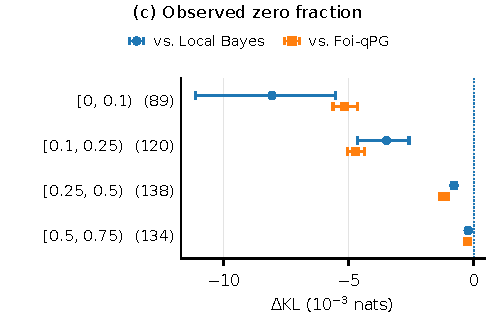
\includegraphics[width=0.493\textwidth]{f10c_holdout_zeros.pdf}\hfill
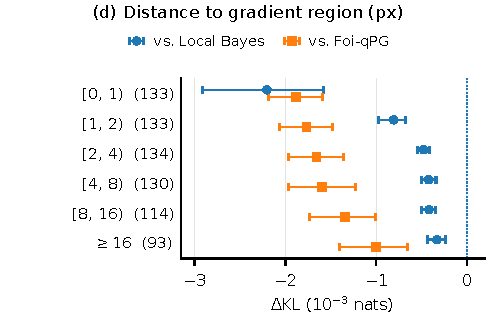
\includegraphics[width=0.493\textwidth]{f10d_holdout_gradient.pdf}
\caption{留出测试集（256 像素上下文）的分区域超额 KL 差值。点与误差条表示 N0 减 Local Bayes（圆点）或 Foi-qPG（方点）的均值差及 95\% 源图 bootstrap 区间，负值表示 N0 误差更低，括号内为源图数。（a）、（b）、（d）的特征来自模拟信号，（c）的零码比例来自输入 RAW（补充材料第~\ref{sec:regionaldefinitions} 节）。}
\label{fig:spatial}
\end{figure*}

\subsection{空间信息的作用}
\subsubsection{跨 CFA 信息}
局部估计器也可在不构建多尺度网络的情况下联合利用四个 CFA 相位。在 32 幅开发源图的 32,462 个共同位置上，Joint-CFA Bayes、同相位 Local PG 与 N0 的平均超额 KL 分别为 0.001790969、0.001952344 和 0.000376673 nats（补充表~\ref{tab:joint}）。N0 显著优于该四相局部对照，但两者除 CFA 通道外还存在感受野范围与先验容量的差异。

\subsubsection{位置分配}
为区分预测分布的整体集合构成与空间位置匹配，我们在各开发源图及各 CFA 相位内部随机置换删失位置上的预测信号，保持校准常量与预测分布集合完全不变。

仅这一空间打乱就使 32 幅开发源图的平均超额 KL 从 0.0003719 升至 0.0026373 nats（原位置减置换的成对差值为 $-0.0022654$ nats，95\% 区间 $[-0.0034895,-0.0012476]$），证明将每个预测分布精确分配到对应的空间像素是补全精度的核心来源。

\subsubsection{绝对误差与信号匹配对比}\label{sec:gradientcontrol}
高梯度区域中两类估计器的绝对误差均上升，但 Local PG 恶化幅度大得多。在 32 幅开发源图中，低梯度组 N0 与 Local PG 的平均超额 KL 为 $0.000191$ 对 $0.000791$ nats，高梯度组则升至 $0.000442$ 对 $0.002109$ nats。成对 KL 差（N0 减 Local PG）从低梯度到高梯度的平均变化量为 $-0.001066$ nats（中位数 $-0.000102$，32 幅中 23 幅为负）。在同源图、同 CFA 相位和粗信号分箱内严格匹配后，27 幅有效源图上的平均差值变化量仍达 $-0.000268$ nats（详细匹配规则与 NLL 结果见补充材料第 IV 节）。

\subsection{校准与模型失配}
N0 的 90\% 等尾整数预测区间覆盖了留出测试码的 91.817\%，与已知信号参考的 91.853\% 一致。鉴于离散整数区间的实际概率质量常略高于标称水平，补充表~\ref{tab:coverage} 给出了四个分位水平下经验覆盖率与区间预测概率质量的对比。

在扰动读出噪声（$\pm10\%$）或叠加未建模高斯行列条带偏移的六种开发集失配条件下，N0 的平均 NLL 与 CRPS 均持续低于 Local PG（补充图~\ref{fig:pairedstress}）。

\subsection{真实传感器读出的条件分布}
两次 2400 万像素暗室曝光 P2654748 和 P2654749 保留了标称黑电平以下的有符号传感器码。利用十幅独立暗帧标定的逐相位整数平移构造真实隐藏读出 $V$，各方法仅接收截零后的观测 $Y=\max(V,0)$（坐标变换与残余小数偏移见补充材料第 V 节）。

每次曝光在六个固定感兴趣区域（ROI）内评估，R/$G_1$/$G_2$ 主评测集分别包含 12,652 和 19,200 个删失位置。B 相位仍参与四相网络输入与抽样 Bayer 输出，但因其传感器暗帧统计与 R/$G_1$ 存在差异，其评分仅作诊断。实拍评估中局部基线采用 $3\times3$ 同相位窗口。

\begin{table}[t]
\centering\footnotesize
\setlength{\tabcolsep}{3pt}
\caption{真实有符号读出案例研究。每次曝光使用共享 R/$G_1$/$G_2$ 候选项与固定实拍方案。NLL 单位为每候选项 nats，CRPS 单位为 DN（数值越低越好）。}
\label{tab:real}
\begin{tabular}{@{}lrrrr@{}}
\toprule
& \multicolumn{2}{c}{P2654748} & \multicolumn{2}{c}{P2654749}\\
\cmidrule(lr){2-3}\cmidrule(l){4-5}
方法 & NLL & CRPS & NLL & CRPS\\
\midrule
Global PMF & 3.980276 & 8.289612 & 4.005568 & 8.347404\\
Global PG & 3.979631 & 8.283446 & 4.004966 & 8.341612\\
Local PG & 3.975846 & 8.248081 & 4.004176 & 8.331820\\
Local Bayes & 3.978475 & 8.273926 & 4.006270 & 8.352316\\
Foi-qPG & 3.979516 & 8.283580 & 4.006041 & 8.350880\\
\textbf{N0/PG} & \textbf{3.974503} & \textbf{8.237064} & \textbf{4.003213} & \textbf{8.322619}\\
\bottomrule
\end{tabular}
\end{table}

如表~\ref{tab:real} 所示，在 P2654748 和 P2654749 中，N0 相对 Local PG 的平均 NLL 分别改善 0.001342 和 0.000964 nats，CRPS 分别改善 0.011017 和 0.009200 DN。第一次曝光中 N0 在六个 ROI 中的五个取得更低 NLL，第二次曝光中为六个中的两个（补充材料第~\ref{sec:realcode} 节）。

同时，校准 PG 模型显著低估了真实读出的极端负尾。在全部 31,852 个候选位置中，$V\leq-128$、$V\leq-256$、$V\leq-305$ DN 的实际观测次数分别为 122、21、13，而高斯读噪尾部预测次数仅为 $9.01\times10^{-3}$、$3.76\times10^{-20}$、$8.63\times10^{-30}$。尽管如此，剔除深尾事件或重复坐标后，N0 相对 Local PG 的成对 NLL 优势依然稳健保持（补充表~\ref{tab:real_robust}）。

\subsection{对去马赛克与暗部颜色的影响}\label{sec:downstream}
\subsubsection{真实曝光的去马赛克统计}
为检验前端补全如何影响常规插值，我们使用同一 LibRaw AHD 实现对保留的有符号参考、截零输入、N0 样本及 Local PG 样本执行去马赛克。通过在无符号 LibRaw 接口前统一加上 512 DN 数字基座并在颜色处理前从线性相机 RGB 中扣回，负向读出得以完整参与插值。

对每个区域的 32 个条件抽样样本分别去马赛克并计算空间统计量，再跨抽样取平均。在 P2654748 最暗 ROI 中，截零使线性 G 均值从 9.003 升至 16.322 DN，N0 与 Local PG 分别将其恢复至 8.621 和 8.602 DN。同时，色差 $R-G$ 的空间标准差因截零从 25.986 降至 18.635 DN，经 N0 与 Local PG 抽样后分别恢复至 25.157 和 25.256 DN。条件抽样恢复了被删失消除的大部分暗部起伏，且两种估计器的统计结果高度接近（补充表~\ref{tab:ahd}、补充材料第 V 节及 \href{visual_zh.pdf}{补充图像 A}）。

\subsubsection{合成场景中基于无噪参考的暗部颜色误差}
另一项受控开发集实验进一步评估补全对渲染后暗部色彩的影响。八幅自然场景和四个程序化模板依次经过 AHD、四倍有符号域平均，以及固定白平衡、色彩转换和曝光缩放，并以去马赛克后的量化无噪信号 $Q(s)$ 为参考，在线性显示 RGB 中计算块均值色度 $(R-G,B-G)$ 的平方误差（补充材料第~\ref{sec:cleanendpoint} 节）。

在八幅自然场景中，直接截零使暗部颜色误差从有符号读出的 0.125006 激增至 1.257683（表~\ref{tab:cleanendpoint}）。条件抽样将该误差拉回有符号参考水平，其中 N0 为 0.122891，Local PG 为 0.126031，成对差值（N0 减 Local）为 $-0.00314$（95\% 源图 bootstrap 区间 $[-0.00614,-0.00084]$，相对降幅 2.49\%）。改用量化条件均值（均值-$Q$）可将误差进一步降至 0.102618（N0）和 0.105440（Local PG）。

\begin{table}[t]
\centering\small
\setlength{\tabcolsep}{4pt}
\caption{八幅自然开发源图的暗部颜色误差与干净 RAW MSE（源图等权汇总）。颜色误差为曝光缩放线性显示 RGB 中块均值 $(R-G,B-G)$ 的平方误差，RAW MSE 以 $Q(s)$ 为参考且单位为 DN$^2$。原始有符号输入为未删失含噪读出。两项指标均越低越好。}
\label{tab:cleanendpoint}
\begin{tabular}{@{}lrr@{}}
\toprule
RAW 输入 & 暗部颜色误差 & RAW MSE\\
\midrule
原始有符号 & 0.125006 & 1157.747\\
直接钳位 & 1.257683 & \textbf{866.698}\\
Local PG 抽样 & 0.126031 & 1157.244\\
N0/PG 抽样 & \textbf{0.122891} & 1159.305\\
Local PG 均值-$Q$ & 0.105440 & 1077.675\\
N0/PG 均值-$Q$ & \textbf{0.102618} & 1076.179\\
\bottomrule
\end{tabular}
\end{table}

表~\ref{tab:cleanendpoint} 中两列指标的相反排序源于其评价目标的差异。对非负干净参考 $c=Q(s)$ 和任意允许填充值 $k\leq0$，恒有 $(k-c)^2-c^2=k^2-2kc\geq0$。因此在保持正码不变的约束下，零填充（$k=0$）在代数上必然最小化逐像素干净 RAW MSE，却因抬高暗部均值而在去马赛克后产生最大的块颜色误差，而量化条件均值则在该固定渲染管线下取得最低色彩误差。

\subsection{运行时间与全分辨率推理}\label{sec:runtime}
在 RTX 3090 Ti 上，N0/PG 完成 2400 万像素读出补全的中位耗时为 27.3901 s，Local PG 为 205.1503 s，CUDA 峰值已分配显存分别为 750.69 与 94.84 MiB（两套数值后端的实现条件见补充表~\ref{tab:runtime}）。全分辨率推理采用相位对齐的重叠分块（补充材料第 VI 节），坐标索引抽样确保固定条件分布下的采样结果与分块顺序无关（补充材料第 III 节）。

\section{讨论}
留出实验表明，条件读出补全的精度直接取决于预测分布所处的空间位置。在边缘与纹理等信号变化剧烈的区域，局部常值模型误差显著上升，多尺度估计的优势尤为突出。反之，在保持预测分布集合不变的前提下打乱其空间位置会使超额 KL 大幅恶化，证实空间位置分配是条件补全精度的核心来源。

恰当概率评分衡量条件读出分布本身的估计精度，而下游图像统计还受去马赛克与色彩处理的影响。匹配物理模型下的合成实验借助已知信号参考剥离了固有读出噪声熵。在实拍曝光中，尽管共享的高斯读噪模型严重低估了罕见极端负码，N0 仍保持稳健的成对似然优势。两类条件抽样方法均恢复了去马赛克暗部起伏，而受控渲染实验进一步表明，零填充虽在数学上最小化干净 RAW MSE，却会造成显著的暗部色度偏差。

\section{结论}
下限删失 RAW 图像中的每个零码都隐藏着非正整数读出的离散条件分布。N0/PG 利用多尺度四相 Bayer 上下文与校准量化 PG 解码器估计各位置的条件分布，仅在删失位置抽样并原样保留所有正码。在 138 幅留出源图上，该方法一致优于全局、局部似然与变换域基线，而实拍有符号读出与固定渲染实验进一步展示了恢复缺失负码对保持暗部统计与色彩的作用。

\section*{可复现性声明}
随附仓库提供表格评分、源图标识、色彩评价记录、冻结模型权重及推理与评测脚本，并已在隔离环境中通过验证与 SHA-256 清单核对。原创代码与权重采用 MIT 许可，原创图表与数值结果采用 CC BY 4.0，第三方材料保留各自许可。

\begin{thebibliography}{10}
\fontsize{7.8}{8.1}\selectfont
\setlength{\itemsep}{0pt}
\bibitem{foi2008} A. Foi, M. Trimeche, V. Katkovnik, and K. Egiazarian, ``Practical Poissonian--Gaussian noise modeling and fitting for single-image raw-data,'' \emph{IEEE Transactions on Image Processing}, vol. 17, no. 10, pp. 1737--1754, 2008. doi: 10.1109/TIP.2008.2001399.
\bibitem{foi2009} A. Foi, ``Clipped noisy images: Heteroskedastic modeling and practical denoising,'' \emph{Signal Processing}, vol. 89, no. 12, pp. 2609--2629, 2009. doi: 10.1016/j.sigpro.2009.04.035.
\bibitem{mathworksISP} MathWorks, ``End-to-End Implementation of a Digital Camera Processing Pipeline,'' Image Processing Toolbox documentation, accessed 28 October 2026. \url{https://ww2.mathworks.cn/help/images/end-to-end-implementation-of-digital-camera-processing-pipeline.html}
\bibitem{librawD5300} LibRaw technical support, ``Nikon NEF RAW Data Minimum Value Clamp: D5300 Code-Floor Investigation,'' 2018. \url{https://www.libraw.org/node/2362}
\bibitem{claffReadNoise} B. Claff, ``Read Noise: The Effect of Black Clipping in Nikon D70 Dark Frames,'' Photons to Photos, prepared 25 November 2007, accessed 28 October 2026. \url{https://photonstophotos.net/GeneralTopics/Sensors_&_Raw/Read_Noise.htm}
\bibitem{aim2025Video} A. Yakovenko, G. Chakvetadze, I. Khrapov, M. Zhelezov, D. Vatolin, R. Timofte, et al., ``AIM 2025 Low-light RAW Video Denoising Challenge: Dataset, Methods and Results,'' in \emph{Proc. IEEE/CVF ICCV Workshops}, pp. 5703--5713, 2025. \url{https://arxiv.org/html/2508.16830}
\bibitem{sonyAIM2025} Sony Research, ``AIM 2025 Challenge on Low-Light Real-World RAW Image Denoising Using Synthetic Data: Official Starter Kit,'' 2025. \url{https://github.com/SonyResearch/AIM2025_Denoise_Challenge/blob/main/README.md}
\bibitem{nafnet} L. Chen, X. Chu, X. Zhang, and J. Sun, ``Simple baselines for image restoration,'' in \emph{European Conference on Computer Vision}, 2022, pp. 17--33. doi: 10.1007/978-3-031-20071-7\_2.
\bibitem{oneill2024} E. O'Neill, ``Type I Tobit Bayesian additive regression trees for censored outcome regression,'' \emph{Statistics and Computing}, vol. 34, art. 123, 2024. doi: 10.1007/s11222-024-10434-4.
\bibitem{kodgirwar2024} S. Kodgirwar, L. Loetgering, C. Liu, A. Joseph, L. Licht, D. S. Penagos Molina, W. Eschen, J. Rothhardt, and M. Habeck, ``Bayesian multi-exposure image fusion for robust high dynamic range ptychography,'' \emph{Optics Express}, vol. 32, no. 16, pp. 28090--28099, 2024. doi: 10.1364/OE.524284.
\bibitem{wei2020} K. Wei, Y. Fu, J. Yang, and H. Huang, ``A physics-based noise formation model for extreme low-light raw denoising,'' in \emph{IEEE/CVF Conference on Computer Vision and Pattern Recognition}, 2020, pp. 2758--2767. doi: 10.1109/CVPR42600.2020.00283.
\bibitem{zhang2021} Y. Zhang, H. Qin, X. Wang, and H. Li, ``Rethinking noise synthesis and modeling in raw denoising,'' in \emph{Proceedings of the IEEE/CVF International Conference on Computer Vision}, 2021, pp. 4593--4601. doi: 10.1109/ICCV48922.2021.00455.
\bibitem{mohammadi2026} M. Mohammadi, S. Honari, S. Tsogkas, T. Aumentado-Armstrong, M. S. Brown, I. Mohomed, K. G. Derpanis, A. Levinshtein, and I. Gilitschenski, ``Why low-light cameras go color blind: Removing color bias in raw denoising,'' \emph{arXiv preprint arXiv:2607.11090}, 2026.
\bibitem{gilton2021} D. Gilton, G. Ongie, and R. Willett, ``Deep equilibrium architectures for inverse problems in imaging,'' \emph{IEEE Transactions on Computational Imaging}, vol. 7, pp. 1123--1133, 2021. doi: 10.1109/TCI.2021.3118944.
\bibitem{goujon2023} A. Goujon, S. Neumayer, P. Bohra, S. Ducotterd, and M. Unser, ``A neural-network-based convex regularizer for inverse problems,'' \emph{IEEE Transactions on Computational Imaging}, vol. 9, pp. 781--795, 2023. doi: 10.1109/TCI.2023.3306100.
\bibitem{bohra2022} P. Bohra, T.-a. Pham, J. Dong, and M. Unser, ``Bayesian inversion for nonlinear imaging models using deep generative priors,'' \emph{IEEE Transactions on Computational Imaging}, vol. 8, pp. 1237--1249, 2022. doi: 10.1109/TCI.2023.3236155.
\bibitem{gnanasambandam2024} A. Gnanasambandam, Y. Sanghvi, and S. H. Chan, ``The secrets of non-blind Poisson deconvolution,'' \emph{IEEE Transactions on Computational Imaging}, vol. 10, pp. 343--356, 2024. doi: 10.1109/TCI.2024.3369414.
\bibitem{gneiting2007} T. Gneiting and A. E. Raftery, ``Strictly proper scoring rules, prediction, and estimation,'' \emph{Journal of the American Statistical Association}, vol. 102, no. 477, pp. 359--378, 2007. doi: 10.1198/016214506000001437.
\bibitem{gharbi2016} M. Gharbi, G. Chaurasia, S. Paris, and F. Durand, ``Deep joint demosaicking and denoising,'' \emph{ACM Transactions on Graphics}, vol. 35, no. 6, pp. 191:1--191:12, 2016. doi: 10.1145/2980179.2982399.
\bibitem{hirakawa2005} K. Hirakawa and T. W. Parks, ``Adaptive homogeneity-directed demosaicing algorithm,'' \emph{IEEE Transactions on Image Processing}, vol. 14, no. 3, pp. 360--369, 2005. doi: 10.1109/TIP.2004.838691.
\bibitem{libraw} LibRaw contributors, ``LibRaw 0.22.1, pinned source revision b860248a89d9082b8e0a1e202e516f46af9adb29,'' software source, accessed 27 October 2026. \url{https://github.com/LibRaw/LibRaw/tree/b860248a89d9082b8e0a1e202e516f46af9adb29}
\bibitem{jot} JOT measurement resource, ``Photon-transfer measurement record: Panasonic S5 II, ISO12800, mechanical shutter,'' archived measurement resource, 2026. \url{https://y-g-jiang.github.io/JOT.html}
\bibitem{div2k} E. Agustsson and R. Timofte, ``NTIRE 2017 challenge on single image super-resolution: Dataset and study,'' in \emph{IEEE Conference on Computer Vision and Pattern Recognition Workshops}, 2017, pp. 126--135. doi: 10.1109/CVPRW.2017.150.
\bibitem{bsds500} P. Arbeláez, M. Maire, C. Fowlkes, and J. Malik, ``Contour detection and hierarchical image segmentation,'' \emph{IEEE Transactions on Pattern Analysis and Machine Intelligence}, vol. 33, no. 5, pp. 898--916, 2011. doi: 10.1109/TPAMI.2010.161.
\bibitem{bm3d} K. Dabov, A. Foi, V. Katkovnik, and K. Egiazarian, ``Image denoising by sparse 3-D transform-domain collaborative filtering,'' \emph{IEEE Transactions on Image Processing}, vol. 16, no. 8, pp. 2080--2095, 2007. doi: 10.1109/TIP.2007.901238.
\end{thebibliography}
\end{document}
